\hinttext{!!!ACTION REQUIRED!!!}
\hinttext{From this point forward until the conclusion, everything becomes pretty individual. The structure I defined is generic and will most likely have to be adapted. I suggest that you skim through the pages and then clear the files \texttt{text/ch2.tex} to \texttt{text/ch7.tex} before you start writing.}

\noindent The beginning of each section should start with a paragraph that tells the reader how the chapter is organized.

\section{First Background Topic}
\label{s:First-Background-Topic}

Provide background information that will help potential readers to understand your research. It is up to you to decide the volume and content of this chapter.

At the time you start writing your thesis you have probably already published novel works and become an expert in your field of research. You may find it difficulty to assume the perspective of a less experienced reader.

Your potential audience is predominately academic and works on tangentially related things. Thus, you may assume that a typical reader has successfully completed all compulsory undergraduate-degree subjects for a related degree. For example, if you do a PhD in computer science or a related discipline, you may assume that the reader knows what the difference between the declarative and imperative programming paradigm is, or what the difference between a linked-list and a tree is.

\section{Second Background Topic}
\label{s:Second-Background-Topic}

Are there people in your department that teach an elective or graduate-level subject that relates to your field of research? If yes, check how they structure their lecture! Tap into the knowledge of the more experienced people around you. Discuss with your supervisors or research coordinator what background information they regard as relevant. Sometimes, they may have a very clear idea.

\section{Grammar Checking}
While overleaf includes a spellcheck function, it doesn't include grammar checking. Installing a browser plugin such as \href{https://www.overleaf.com/blog/635-languagetool-a-free-browser-add-on-to-check-your-grammar-and-spelling}{language tools}
 is the best way to overcome this. 
\section{Acronym Example}\label{sec:acro_example}


In the early nineties, \acs{GSM} was deployed in many European countries. \ac{GSM} offered for the first time international roaming for mobile subscribers. The \acs{GSM}’s use of \ac{TDMA} as its communication standard was debated at length. And every now and then there are big discussion whether \ac{CDMA} should have been chosen over \ac{TDMA}.

\section{Python Plotting Examples}

The Jupyter notebook can be found in the folder 'Python plotting example' and contains code and advice for plotting publication quality figures for your thesis using python. View this notebook without installing python \href{https://nbviewer.jupyter.org/github/blairium/ltu-thesis/blob/97c95023caed8c8055ad905a8f68ad73061df8ad/Python_plotting_example/Plotting_Example.ipynb}{here}.



\begin{figure}[H]
    \centering
    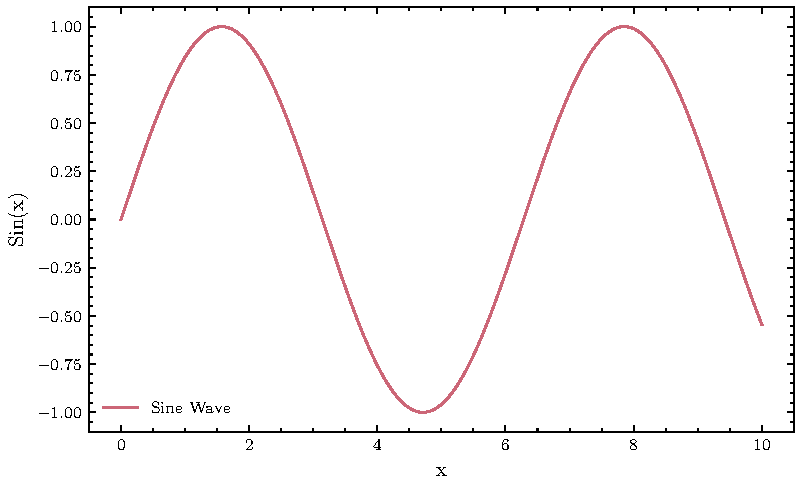
\includegraphics{Python_plotting_example/example_1.pdf}
    \caption[Python example plot 1]{Python example plot 1, a simple sine plot.}
    \label{fig:ch2/example_1}
\end{figure}
\begin{figure}[h!]
    \centering
    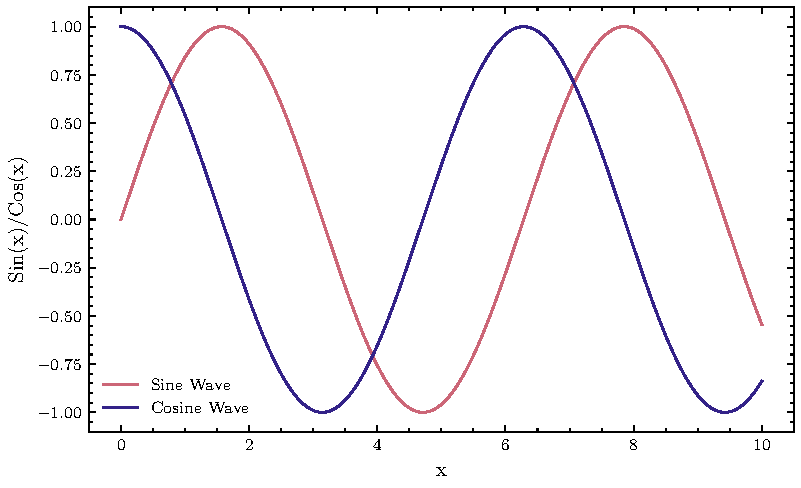
\includegraphics{Python_plotting_example/example_2.pdf}
    \caption[Python example plot 2]{Python example plot 2, a sine and cosine plot.}
    \label{fig:ch2/example_2}
\end{figure}
\begin{figure}[h!]
    \centering
    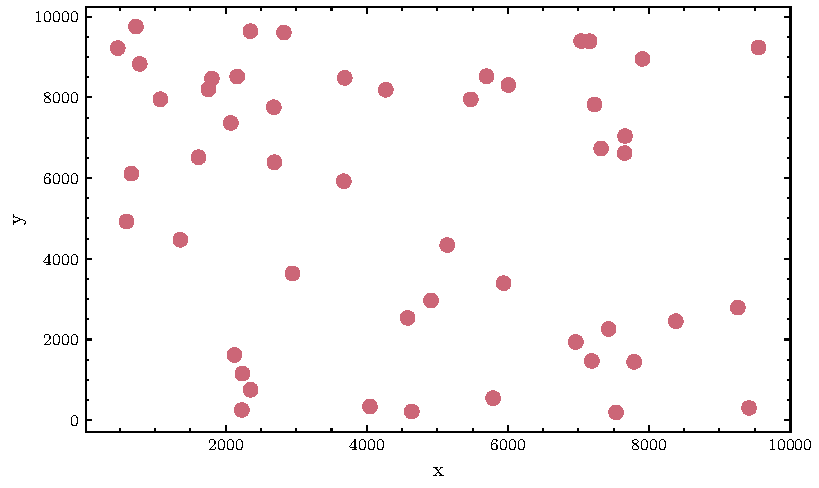
\includegraphics{Python_plotting_example/example_3.pdf}
    \caption[Python example plot 3]{Python example plot 3, a scatter plot of random data.}
    \label{fig:ch2/example_3}
\end{figure}
\begin{figure}[h!]
    \centering
    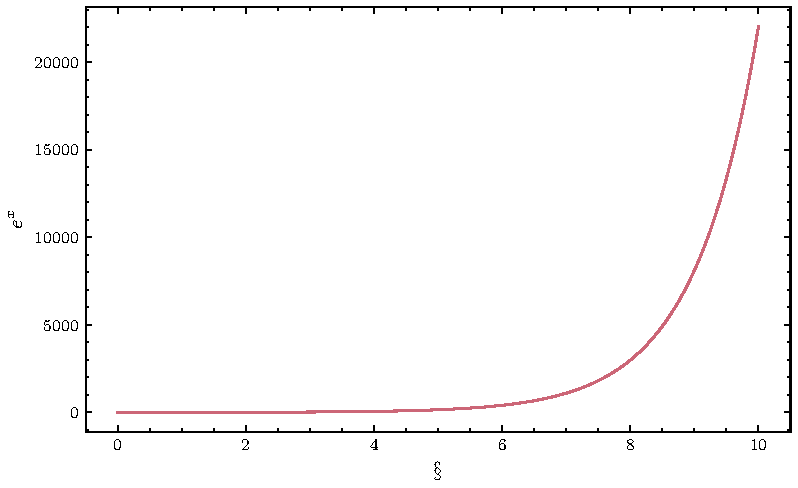
\includegraphics{Python_plotting_example/example_4.pdf}
    \caption[Python example plot 4]{Python example plot 4, an exponential plot showing how tex can be used within python.}
    \label{fig:ch2/example_4}
\end{figure}



\section{Chem Example}
%https://mirror.aarnet.edu.au/pub/CTAN/macros/latex/contrib/mhchem/mhchem.pdf

\ce{H2O}

\ce{H2O} is water. \ce{2H2 + O2 <-> 2H2O}

\ce{Hg^2+ ->[I-] HgI2
->[I-] [Hg^{II}I4]^2-}

\begin{align}
    \ce{2H2& + 2O &-> 2H2O} \\
   \ce{2F2& + 2H &-> 2HFe2O}
\end{align}

\ce{Hg^2+ ->[I-] HgI2
->[I-] [Hg^{II}I4]^2-}

\section{Math Example}
Math requires the use of a special environment, with between single \$'s for inline math like $2^2=4$, or between double \$\$'s for on it's own line like $$2^3=8$$ Math mode is also required to use the \href{https://mirror.aarnet.edu.au/pub/CTAN/macros/latex/contrib/siunitx/siunitx.pdf}{siunitx} package to produce standardised units like $\SI{1.23}{\percent\per\milli\litre}$

$\SI{123}{\degree\per\pico\litre}$

    \begin{math}
        2^3=8
    \end{math}
    
    \begin{align}
        27 &= 3^3 \\
        &= 9 \times 9
    \end{align}
\section{Section Example}\label{sec:section_Example}
\subsection{Subsection Example}
\subsubsection{Subsubsection Example}
    
    
\section{Tables Examples}
Unlike figures and the standard table environment, the longtable package will put tables wherever you put them, so you might have to play around with their location. Tables are without a doubt the most annoying aspect of \LaTeX. A helpful tool which can convert Excel tables to latex tables can be found \href{https://github.com/krlmlr/Excel2LaTeX}{here}.

\newpage %This command forces the table to the next page
\subsection{Portrait Table}
%This is a normal portrait table


\begin{longtable}{@{}l *{2}{rr}}
\caption[Portrait Table, short caption]{Portrait Table example:, long caption}
\label{table:portrait_table}
\\
%   
\toprule%


 {\bfseries Sample} & {\bfseries Number } & {\bfseries Number}  
\\



\cmidrule[0.4pt](r{0.125em}){1-1}%
\cmidrule[0.4pt](lr{0.125em}){2-3}%
\cmidrule[0.4pt](lr{0.125em}){4-5}%


  \endfirsthead

\endhead



Sample & 1& 2
\\

\myrowcolour%
Sample & 1 & 2
\\
Sample & 1 & 2
\\


\bottomrule

\end{longtable} %Here we input our table from a separate file to keep tings neat. As you can see, longtable will flow over pages so be careful where you put it or use the regular tabular environment
% https://www.overleaf.com/learn/latex/Tables

\subsection{Landscape Table}
%This creates a landscape table, perfect for wide tables

\afterpage{%
    \clearpage% Flush earlier floats (otherwise order might not be correct)
    \thispagestyle{empty}% empty page style (?)
    \begin{landscape}% Landscape page

\begin{longtable}{@{}l*{7}{ll}}
\caption[Landscape table short caption]{Landscape table example: long caption}
\label{table:/Chapter2/landscape}
\\

\toprule%


{\bfseries Number } &  & {\bfseries Value 1 } &  &{\bfseries Value 2 } & & {\bfseries Value 3 } &  & {\bfseries Value 4 } & & {\bfseries Value 5 } & & {\bfseries Value 6 } &  &{\bfseries Value 7 } \\



\cmidrule[0.4pt](r{0.125em}){1-1}%
\cmidrule[0.4pt](lr{0.125em}){2-3}%
\cmidrule[0.4pt](lr{0.125em}){4-5}%
\cmidrule[0.4pt](lr{0.125em}){6-7}%
\cmidrule[0.4pt](lr{0.125em}){8-9}%
\cmidrule[0.4pt](lr{0.125em}){10-11}%
\cmidrule[0.4pt](lr{0.125em}){12-13}%
\cmidrule[0.4pt](lr{0.125em}){14-15}%


  \endfirsthead

\endhead



1  & Value & $\SI{5}{\nano\m}$ & Value & $\SI{5}{\nano\m}$  &  Value  & $\SI{5}{\nano\m}$ 
 & Value & $\SI{5}{\nano\m}$ & Value  & $\SI{5}{\nano\m}$ &   &  
\\

\myrowcolour%
2  & Value &  $\SI{5}{\nano\m}$  & Value & $\SI{5}{\nano\m}$  &  Value & $\SI{5}{\nano\m}$  & Value &
$\SI{5}{\nano\m}$  & Value & $\SI{5}{\nano\m}$   & Value & $\SI{5}{\nano\m}$  & Value & $\SI{5}{\nano\m}$
\\


3 & Value & $\SI{5}{\nano\m}$ & Value  & $\SI{5}{\nano\m}$  &  Value  & $\SI{5}{\nano\m}$ & Value &
$\SI{5}{\nano\m}$  &  &   &   &  
\\
\myrowcolour%
4  & Value &  $\SI{5}{\nano\m}$  & Value & $\SI{5}{\nano\m}$ &  Value & $\SI{5}{\nano\m}$  &
  &   &  &   &    &   &  &   
\\


\bottomrule

\end{longtable}

\end{landscape}
    \clearpage% Flush page
}

\section{Summary}
\label{s:Background-Summary}

The final section of each chapter should summarize the chapter. In comparison to the chapter, the summary should be short ($\frac{1}{2}$ to $2$ pages is normal).

Example beruwoeruioh \cite{HerbertF:1965:Dune} \citeauthor{HerbertB:2002:Butlerian-Jihad} \citeyear{HerbertB:2000:Harkonnen}

